\chapter{Introducere}
\label{chap:intro}

\section{Motivația alegerii temei}
Transportul și distribuția apei reprezintă una dintre cele mai vechi preocupări inginerești de proporții, existând de mai mult de 4000 de ani. Civilizația minoică, localizată în insula Creta, este considerată a fi prima care a construit apeducte - structuri pentru transportul apei de la sursă către orașe - în 2500 î.Hr. 

Deși majoritatea popoarelor din antichitate care s-au ocupat cu construcția apeductelor întrebuințau aceste sisteme pentru irigația pământului - ocupațiile de bază de atunci fiind în strânsă legătură cu agricultura - romanii au văzut în sistemele de provizionare a apei și un potențial imens în dezvoltarea civilizației, astfel ei sunt ei care aduc cele mai mari contribuții inginerești, apeductele construite de aceștia impresionând și astăzi prin grandoarea și iscusunța cu care au fost construite.

Inovațiile în acest domeniu au suferit salturi bruște și puternice în momentul descoperirii unei noi relații matematice care transformă un parametru despre care se puteau face doar niște estimări grosiere într-o mărime bine definită și bine controlată. Istoric vorbind începutul dezvoltării științei hidraulice s-a bazat pe relația descoperită de Arhimede din Siracuza în sec III î.Hr, $F = V_{obiect} \cdot \rho_{lichid}*g$. O altă contribuție care are o deosebită importanță în domeniul tehnologiei de distribuiție a apei și nu numai o reprezintă tubul lui Pitot folosit la măsurarea vitezei fluidului, inventat de Henri Pitot în sec XVII. Din punct de vedere constructiv tubul are o formă de \textbf{L}, scufundarea acestuia într-un fluid (apă sau gaz) va determina creșterea nivelului și a presiunii până la o anumită limită \cite{klopfenstein1998air}, ecuația care guvernează depedența nivel - viteză este:
\begin{equation}
u = \sqrt{\frac{2(p_t-p_s)}{\rho}} 
\end{equation}

unde:

\begin{description}
\item u reprezintă viteza fluidului;
\item $p_t$ reprezintă presiunea de stagnare;
\item $p_s$ reprezintă presiunea statică;
\item $\rho$ reprezintă densitatea fluidului.
\end{description}

Mergând mai departe, alte contribuții importante apar din partea marilor matematicieni precum Daniel Bernoulli și Leonhard Euler, care au mărit spectrul mecanicii lui Newton și Leibniz spre aria hidraulicii și a termodinamicii. Fluidele considerate sunt incompresibile și au densitatea constantă în timp și uniform distribuită în spațiu. Bernoulli afirmă despre lichidele incompresibile că o creștere în viteză a lichidului este însoțită de o scădere a energiei potențiale a lichidului (i.e. a presiunii):
\begin{equation}
\frac{u^2}{2} + gz + \frac{p}{\rho} = c
\end{equation}

unde:
\begin{description}
\item g reprezintă accelerația la care e supus fluidul;
\item z reprezintă elevația ștrangulației conductei;
\item p reprezintă presiunea într-un anumit punct;
\item $\rho$ reprezintă densitatea fluidului.
\end{description}

În contextul în care se dorește analiza unui caz real este important ca toate diferențele între cazurile ideale și cazurile reale să fie puse în evidență în mod matematic, astfel se particularizează ecuația generală Navier-Stokes pentru cazuri în care se cunosc anumiți parametrii ai sistemului de analizat. Spre exemplu ecuația Poisuille care modelează începutul fluxului de apă într-o conductă este \cite{elger2016engineering}:
\begin{equation}
\frac{\partial u}{\partial t} = \frac{G}{\rho} + \nu \left( \frac{\partial^2 u}{\partial t^2} + \frac{1}{r}\frac{\partial u}{\partial{r}}\right)
\end{equation}

unde:
\begin{description}
\item $u$ reprezintă viteza lichidului prin conductă
\item $t$ reprezintă timpul
\item $G$ reprezintă diferența de presiune
\item $\rho$ reprezintă densitatea lichidului
\item $\nu$ reprezintă vâscozitatea cinematică
\item $r$ reprezintă poziția
\end{description}

Se poate observa că pe măsură ce modelul matematic se apropie de realitate, complexitatea acestuia crește și pentru fiecare situație specială - spre exemplu analiza presiunii la  introducerea apei într-o conductă vs. analiza presiunii când conducta este încărcată cu apă - are nevoie de o ecuație specială sau de o particularizare a ecuației Navier-Stokes, pentru care încă nu se cunoaște dacă există soluții pentru cazul cu 3 dimensiuni și dacă soluțiile acestea sunt netede. 

Ținând cont de importanța apei în desfășurarea activităților cotidiene atât pentru oameni cât și pentru actorii importanți ai industriei, este o condiție absolut necesară ca un oraș să aibă un sistem performant de distribuție a apei. În contextul actual al dezvoltării tehnologiei este natural să folosim tehnici moderne de monitorizare a diferiților parametrii din cadrul unei rețele pentru a putea face o analiză riguroasă și eficientă cu referire nu numai la mentenanță ci și la consumul global și local în ideea îmbunătățirii și reducerii pierderilor.


\section{Expunerea problemei}

În această lucrare se va aborda problematica identificării prezenței unui defect - \textit{Fault detection} și izolarea defectului \textit{Fault isolation} apărut într-un nod al rețelei - aceasta reprezentând o simplificare deoarece un defect apare de obicei într-una din conductele rețelei legate de acel nod. Combinănd cei doi termeni obținem \textit{Fauld detection and Isolation} (FDI).

O rețea de apă poate fi privită ca un graf neorientat $G = (V, E)$ unde $V$ este mulțimea nodurilor rețelei - acestea reprezentând o abstractizare asupra componentelor precum:
\begin{itemize}
\item rezervoare
\item tancuri de apă
\item puncte de distribuție
\end{itemize} 

$E$ este mulțimea muchiilor reprezentând de fapt țevile care fac legătura între noduri.

Mergând mai departe cu abstractizarea se pot considera rețele de apă active și rețele de apă pasive. Diferența între cele două făcându-se în baza pompelor de apă amplasate în zonele unde presiunea sau elevația vin în detrimentul distribuției apei.

Rețelele de apă care vor fi tratate în această lucrare fac parte din categoria pasivă, astfel putem diviza mulțimea nodurilor $V$ în $V^t$ și în $V^j$ reprezentând mulțimea nodurilor de tip tanc și mulțimea nodurilor joncțiune, cu proprietatea că $V = V^t \cup V^j$. Tancurile și rezervoarele dintr-o rețea de apă au proprietatea că nivelul de apă din acestea se va menține la un nivel oarecum staționar, astfel simulările din capitolele viitoare se vor axa pe nodurile simple de tip joncțiune, deci mulțimea de interes în acest caz va fi $V^j$ pentru care cunoaștem cardinalul.

Caracteristicile care se pot recolta dintr-o rețea de apă pot varia în funcție de elementul inspectat și de senzorii dispuși în rețea, astfel pentru fiecare nod $n_i \in V^j$ putem defini la fiecare moment de timp 
\begin{itemize}
\item presiunea $p_i(t)$ - măsurată în metri coloană de apă $mH2O$, mărime influențată puternic de presiunea interioară a nodului și de eventualele perturbații exterioare i.e. scurgeri de apă prin conducte;
\item 'cererea' $d_i(t)$ - măsurată $L/s$, mărime ce caracterizează profilul de utilizare al utilizatorilor de-a lungul unei zile i.e. debitul de apă care ajunge la consumatori. Acest debit poate varia de-a lungul zilei, putem distinge de exemplu intervale de timp în care cererea este foarte mică și rețeaua intră în regim staționar;
\item de asemenea pentru fiecare conductă a rețelei $e_{ij} \in E$ putem măsura viteza lichidului $v_{ij}(t)$.
\end{itemize}



Pentru a putea rezolva problema de FDI este importantă găsirea unei modalități eficiente de selecție și prelucrare a datelor de la rețea.Mai mult, punând în lumină aspectul ingineresc al problemei, trebuie găsită o submulțime $V_{opt} \subset V^j$ ai cărei elemente pot aduce informații necesare și suficiente pentru a detecta un defect într-o acoperire destul de mare a rețelei.

\section{Exemplul de lucru}
În următoarele capitole și în implementarea lucrării consider rețeaua Hanoi iar pentru simularea scenariilor propuse voi folosi biblioteca și suita de funcții \textbf{EPANET} - Environmental Protection Agency NETwork \cite{rossman2000epanet}. 

\noindent Rețeaua Hanoi constă într-o mulțime de noduri de tip joncțiune $V^j$ cu $|V^j| = 31$ și mulțimea $V^t$ cu $|V^t|=1$, ilustrată în figura de mai jos:
 
\begin{figure}[h]
\centering
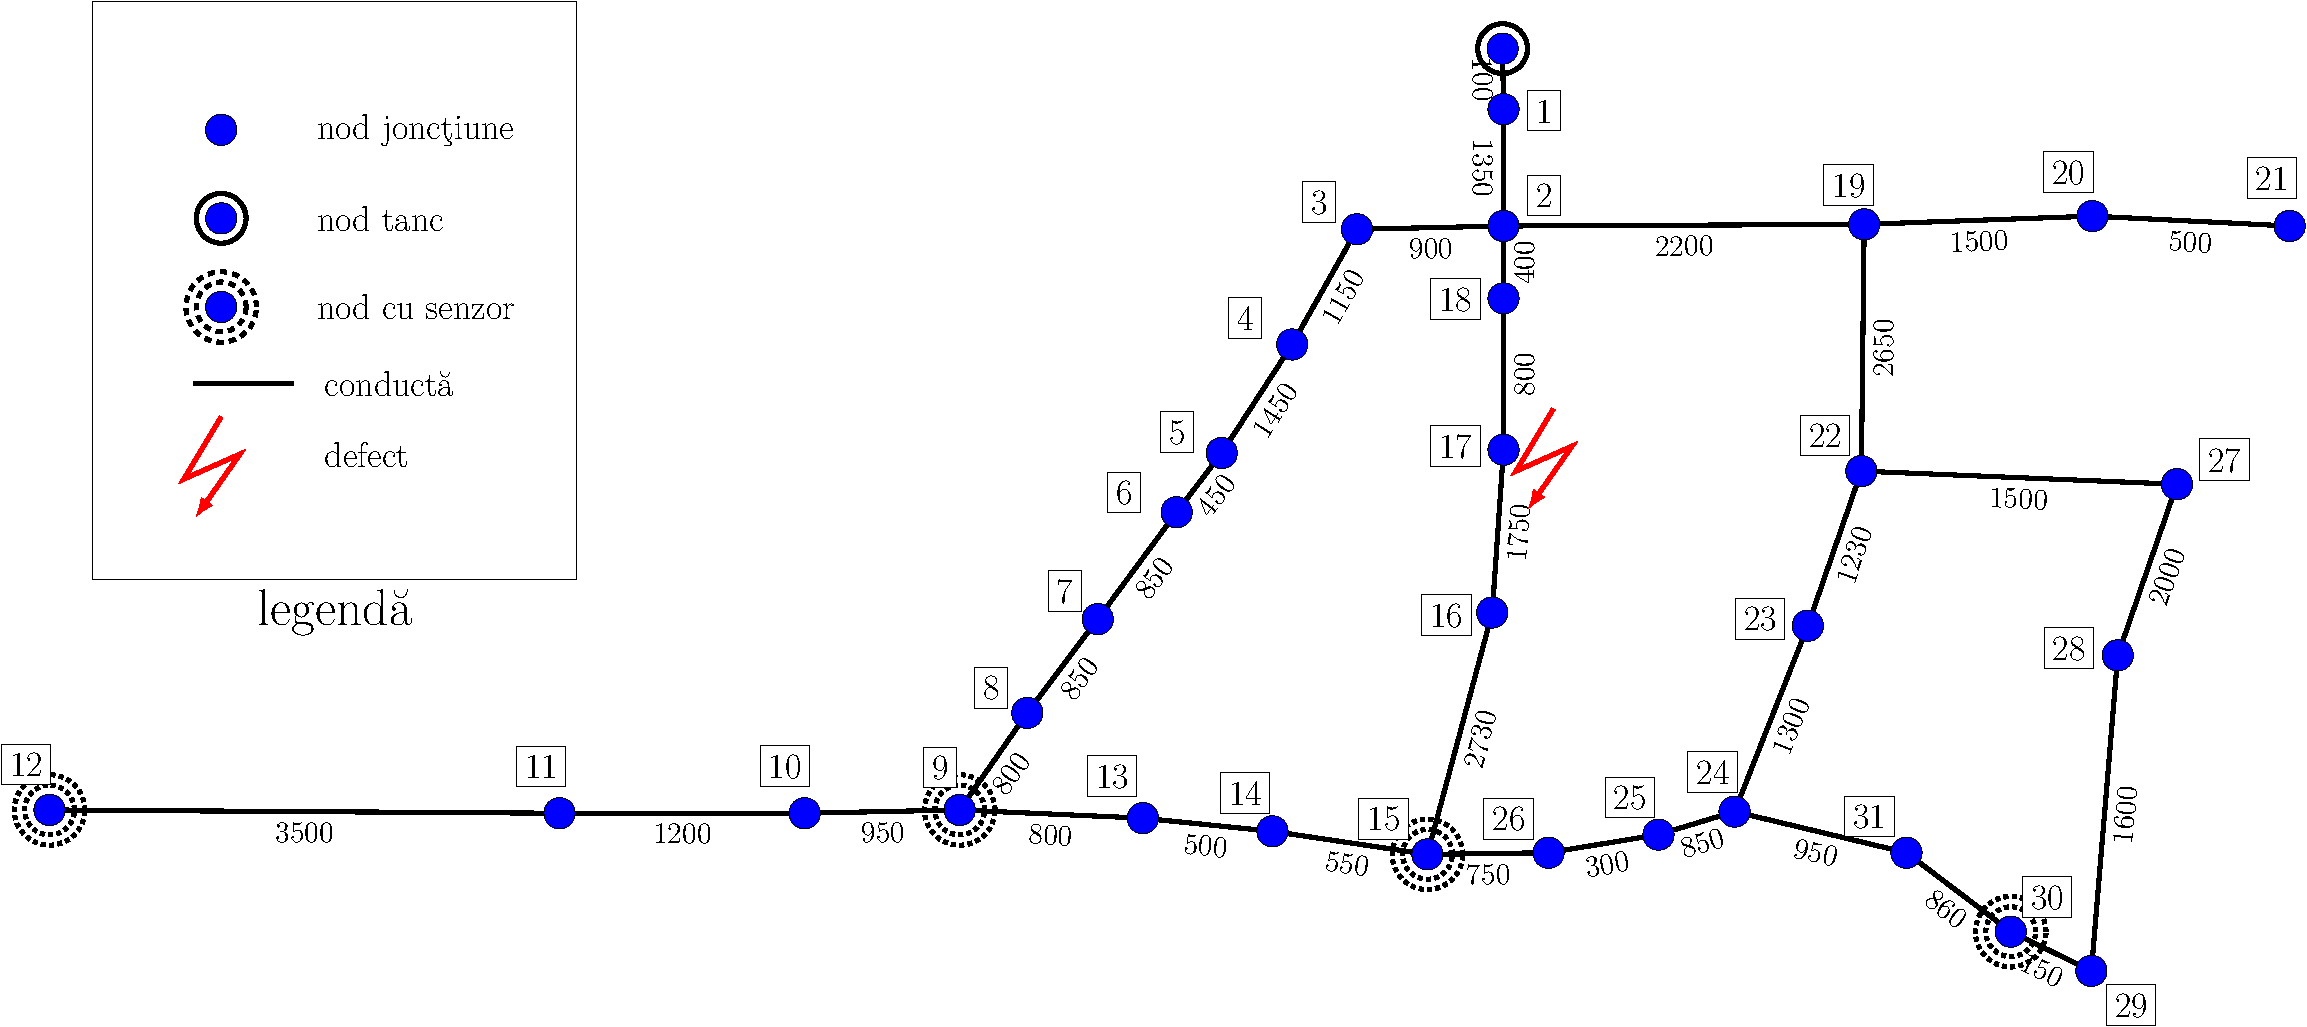
\includegraphics[width=\textwidth]{pics/c1_pics/hanoi_network.pdf}
\caption{Graful rețelei de apă din Hanoi \cite{irofti2017dictionary}}
\label{fig:hanoinetwork}
\end{figure}

După cum se poate observa în figura de mai sus au fost reprezentate două tipuri de node pasive, anume tancurile și joncțiunile. În cazul apariției unui defect în rețea, este important de luat în considerație modalitatea în care acesta va influența valorile apărute în rețea, spre exemplu este de la sine înțeles că dacă se cosideră un defect în nodul cu indicele 17 - i.e. în acest nod au apărut anumite scurgeri care afectează fluxul de apă către consumatori - nodurile în care se va observa o modificare puternică a caracteristicilor (presiune și debit) vor face parte din mulțimea nodurilor adiacente rețelei $S=\{V_{16}, V_{18}\}$, deși pare o concluzie naturală, o modelare matematică riguroasă din care să se tragă această nu este o problemă ușor de rezolvat, anumiți parametrii fiind extrem de greu de estimat chiar și în cazul în care se consideră un regim staționar.
